

\tikzset{every picture/.style={line width=0.75pt}} %set default line width to 0.75pt        

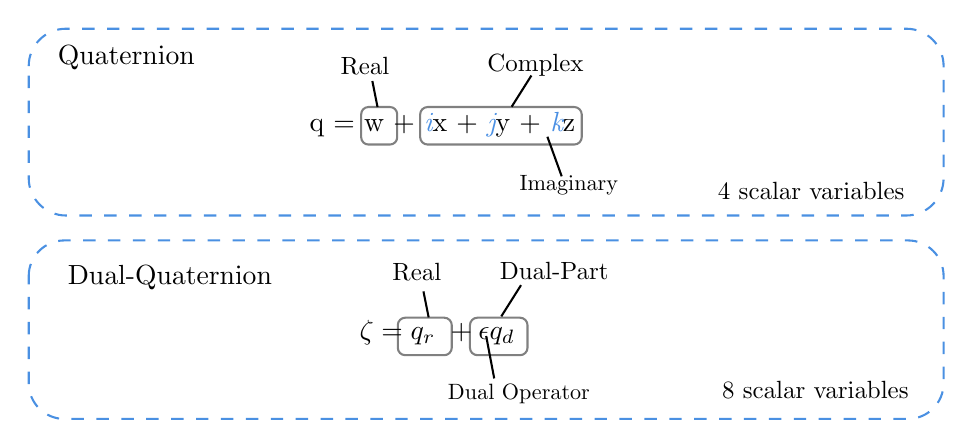
\begin{tikzpicture}[x=0.75pt,y=0.75pt,yscale=-1,xscale=1]
%uncomment if require: \path (0,300); %set diagram left start at 0, and has height of 300

%Rounded Rect [id:dp6466080872798088] 
\draw  [color={rgb, 255:red, 74; green, 144; blue, 226 }  ,draw opacity=1 ][dash pattern={on 4.5pt off 4.5pt}] (100,196.2) .. controls (100,186.7) and (107.7,179) .. (117.2,179) -- (523.59,179) .. controls (533.09,179) and (540.79,186.7) .. (540.79,196.2) -- (540.79,247.8) .. controls (540.79,257.3) and (533.09,265) .. (523.59,265) -- (117.2,265) .. controls (107.7,265) and (100,257.3) .. (100,247.8) -- cycle ;
%Rounded Rect [id:dp7845549288229852] 
\draw  [color={rgb, 255:red, 74; green, 144; blue, 226 }  ,draw opacity=1 ][dash pattern={on 4.5pt off 4.5pt}] (100,95) .. controls (100,85.06) and (108.06,77) .. (118,77) -- (522.79,77) .. controls (532.73,77) and (540.79,85.06) .. (540.79,95) -- (540.79,149) .. controls (540.79,158.94) and (532.73,167) .. (522.79,167) -- (118,167) .. controls (108.06,167) and (100,158.94) .. (100,149) -- cycle ;
%Rounded Rect [id:dp8561511815773608] 
\draw  [color={rgb, 255:red, 128; green, 128; blue, 128 }  ,draw opacity=1 ] (260.19,118.2) .. controls (260.19,116.29) and (261.75,114.73) .. (263.66,114.73) -- (274.06,114.73) .. controls (275.97,114.73) and (277.53,116.29) .. (277.53,118.2) -- (277.53,129.33) .. controls (277.53,131.25) and (275.97,132.8) .. (274.06,132.8) -- (263.66,132.8) .. controls (261.75,132.8) and (260.19,131.25) .. (260.19,129.33) -- cycle ;
%Rounded Rect [id:dp9776560671757293] 
\draw  [color={rgb, 255:red, 128; green, 128; blue, 128 }  ,draw opacity=1 ] (288.59,118.35) .. controls (288.59,116.35) and (290.21,114.73) .. (292.21,114.73) -- (362.84,114.73) .. controls (364.83,114.73) and (366.45,116.35) .. (366.45,118.35) -- (366.45,129.19) .. controls (366.45,131.18) and (364.83,132.8) .. (362.84,132.8) -- (292.21,132.8) .. controls (290.21,132.8) and (288.59,131.18) .. (288.59,129.19) -- cycle ;
%Rounded Rect [id:dp3798019116991682] 
\draw  [color={rgb, 255:red, 128; green, 128; blue, 128 }  ,draw opacity=1 ] (312.59,219.85) .. controls (312.59,217.85) and (314.21,216.23) .. (316.21,216.23) -- (336.7,216.23) .. controls (338.7,216.23) and (340.32,217.85) .. (340.32,219.85) -- (340.32,230.69) .. controls (340.32,232.68) and (338.7,234.3) .. (336.7,234.3) -- (316.21,234.3) .. controls (314.21,234.3) and (312.59,232.68) .. (312.59,230.69) -- cycle ;
%Rounded Rect [id:dp3954108729157688] 
\draw  [color={rgb, 255:red, 128; green, 128; blue, 128 }  ,draw opacity=1 ] (277.82,219.85) .. controls (277.82,217.85) and (279.44,216.23) .. (281.43,216.23) -- (300.2,216.23) .. controls (302.2,216.23) and (303.82,217.85) .. (303.82,219.85) -- (303.82,230.69) .. controls (303.82,232.68) and (302.2,234.3) .. (300.2,234.3) -- (281.43,234.3) .. controls (279.44,234.3) and (277.82,232.68) .. (277.82,230.69) -- cycle ;
%Straight Lines [id:da47919133191646757] 
\draw    (320.4,225.05) -- (324.28,245.5) ;


%Straight Lines [id:da41716187660240633] 
\draw    (337.19,200.55) -- (327.69,215.59) ;


%Straight Lines [id:da0520768716139679] 
\draw    (290.19,203.55) -- (292.69,216.09) ;


%Straight Lines [id:da43941766766200474] 
\draw    (349.9,129.05) -- (356.79,148.11) ;


%Straight Lines [id:da6917573201669784] 
\draw    (342.19,99.55) -- (332.69,114.59) ;


%Straight Lines [id:da8577549839997949] 
\draw    (265.56,102.19) -- (268.06,114.73) ;



% Text Node
\draw (299.33,123) node  [align=left] {q = w + \textit{\textcolor[rgb]{0.29,0.56,0.89}{i}}x + \textit{\textcolor[rgb]{0.29,0.56,0.89}{j}}y + \textit{\textcolor[rgb]{0.29,0.56,0.89}{k}}z};
% Text Node
\draw (296.82,223.27) node  [align=left] {$\displaystyle \zeta =q_{r} \ +\epsilon q_{d}$};
% Text Node
\draw (147,91) node  [align=left] {Quaternion};
% Text Node
\draw (168,197) node  [align=left] {Dual-Quaternion};
% Text Node
\draw (479,251) node [scale=0.9] [align=left] {8 scalar variables};
% Text Node
\draw (477,155) node [scale=0.9] [align=left] {4 scalar variables};
% Text Node
\draw (262,95) node [scale=0.9] [align=left] {Real};
% Text Node
\draw (353.19,193.55) node [scale=0.9] [align=left] {Dual-Part};
% Text Node
\draw (287,194) node [scale=0.9] [align=left] {Real};
% Text Node
\draw (344.19,94.55) node [scale=0.9] [align=left] {Complex};
% Text Node
\draw (360.19,152.55) node [scale=0.8] [align=left] {Imaginary};
% Text Node
\draw (336.19,253.05) node [scale=0.8] [align=left] {Dual Operator};


\end{tikzpicture}